\documentclass{article}
\usepackage{amsmath}
\usepackage{amssymb}
\usepackage{graphicx}
\usepackage{hyperref}
\usepackage[version=4]{mhchem}

\title{Problem 16}
\date{}

\begin{document}
\maketitle

\section*{Problem}
In \(A B C, \angle A C B=90^{\circ}, \angle C A B=30^{\circ}\). with equilateral triangles \(A B E\) and \(A C D\) drawn on sides \(A B\) and \(A C\), respectively. \(D E\) meets \(A B\) at \(F\). Prove: \(E F=F D\).\\
\centering
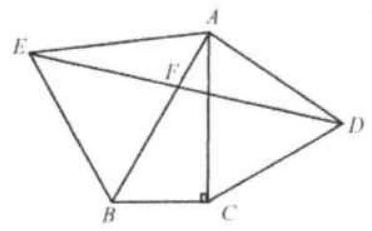
\includegraphics[width=\textwidth]{images/090.jpg}

\section*{Solution}
Solution not available.

\end{document}
